\documentclass[11pt]{article}
\usepackage[a4paper,margin=0.92in]{geometry}
\usepackage{amsmath,amssymb,amsthm,mathtools}
\usepackage{booktabs,array,graphicx,xcolor,xurl,float}
\usepackage[hidelinks]{hyperref}
\hypersetup{pdftitle={Projective Bottlenecks in Passive Spectral Routing},pdfauthor={Lluis Eriksson},pdfsubject={Exact planar memory and unbounded detector gaps}}
\usepackage[nameinlink,capitalise]{cleveref}
\usepackage{microtype,etoolbox}
\AtBeginEnvironment{thebibliography}{\fontsize{8}{9}\selectfont\setlength{\itemsep}{-2pt}\setlength{\parsep}{0pt}}

\newtheorem{theorem}{Theorem}[section]
\newtheorem{lemma}[theorem]{Lemma}
\newtheorem{corollary}[theorem]{Corollary}
\newtheorem{proposition}[theorem]{Proposition}
\theoremstyle{definition}\newtheorem{definition}[theorem]{Definition}\newtheorem{example}[theorem]{Example}
\theoremstyle{remark}\newtheorem{remark}[theorem]{Remark}\newtheorem{limitation}[theorem]{Limitation}
\crefname{lemma}{Lemma}{Lemmas}\crefname{proposition}{Proposition}{Propositions}
\crefname{corollary}{Corollary}{Corollaries}\crefname{limitation}{Limitation}{Limitations}
\crefname{definition}{Definition}{Definitions}\crefname{example}{Example}{Examples}
\crefname{remark}{Remark}{Remarks}
\newcommand{\C}{\mathbb C}\newcommand{\D}{\mathbb D}\newcommand{\T}{\mathbb T}
\newcommand{\PP}{\mathbb P}\newcommand{\rank}{\operatorname{rank}}
\newcommand{\Res}{\operatorname{Res}}\newcommand{\mcdeg}{\deg_{\mathrm{McM}}}
\newcommand{\norm}[1]{\lVert#1\rVert}\newcommand{\dd}{\,\mathrm d}
\newcolumntype{L}[1]{>{\raggedright\arraybackslash}p{#1}}

\title{Projective Bottlenecks in Passive Spectral Routing:\\
Exact Planar Memory, Cross-Ratio Strata, and an Unbounded Detector Gap}
\author{Lluis Eriksson}
\date{13 August 2026}

\begin{document}
\maketitle

\begin{abstract}
We determine the exact passive state cost of every finite routing table whose
target lines lie in one complex two-plane.  At distinct boundary frequencies
$\zeta_i$, a square rational-inner matrix must route one input line to prescribed
target lines $Y_i$.  Let $\delta$ be the least algebraic degree of a rational
map $\PP^1\to\PP^1$ interpolating the ordered projective data
$(\zeta_i,Y_i)$.  We prove the exact reduction
\[
                         d_{\min}=\delta.
\]
The upper bound is constructive: scalar Fej\'er--Riesz factorization lifts any
coprime rational pair to an explicit $2\times2$ lossless network of exactly the
same McMillan degree.  The lower bound uses a common state-space denominator:
more boundary zeros than states force the routed column to remain identically
inside the target plane, where it becomes a projective rational interpolant.

This reduction reveals two competing mechanisms.  For two target lines with
occupancies $n_0,n_\infty$, the exact cost is $\max(n_0,n_\infty)$, a fiber
multiplicity law.  By contrast, for $L$ distinct generic coplanar targets,
\[
             d_{\min}=\left\lceil\frac{L-1}{2}\right\rceil,
\]
whereas both the span bound and the optimized constant-detector hierarchy of
the preceding framework equal one.  Their
multiplicative underestimate is therefore unbounded.  For four nodes we give the
complete phase diagram: degree zero for one constant target, degree one exactly
for four distinct targets with matching ordered cross-ratio, degree three for a
$3+1$ collision, and degree two in every remaining case.  A singular-value
margin makes the algebraic lower certificates stable under perturbation.  Exact
Gaussian-rational fixtures verify all strata, a strict cross-ratio obstruction,
and the generic law through $L=16$.  Exact producer, replay validator, frozen
evidence, and immutable release metadata are linked in the paper.
\end{abstract}

\noindent\textbf{Keywords:} rational inner matrix; projective interpolation;
McMillan degree; passive memory; cross-ratio; Fej\'er--Riesz factorization;
spectral routing; Wigner--Smith delay.

\section{A singular stratum with hidden memory}

Let $S$ be an $N\times N$ rational matrix, analytic in $\D$, unitary almost
everywhere on $\T$, and regular at distinct nodes
$\zeta_1,\ldots,\zeta_L\in\T$.  Its McMillan degree is the state dimension of a
minimal conservative realization.  Fix an input line $X\subset\C^N$ and target
lines $Y_i\subset\C^N$.  The routing task is
\begin{equation}\label{eq:routing}
                              S(\zeta_i)X=Y_i,
                              \qquad 1\le i\le L.
\end{equation}
Endpoint phases and bases are free.  Write $d_{\min}$ for the least McMillan
degree among all such $S$.

The generic direct-sum law counts states by target occupancy, and its
constant-detector extension gives useful lower bounds on singular target
arrangements \cite{ErikssonUnified2026}.  It deliberately leaves open a complete
equality theory outside direct-sum position.  The first unresolved stratum in
that preceding framework is
also the smallest geometrically nontrivial one: all $Y_i$ lie in a fixed
two-plane $H$.  Here the span statistic is frozen, yet projective compatibility
can demand arbitrarily many states.

Classical scalar rational interpolation and its state-variable realization
describe minimal rational functions through finite data
\cite{AntoulasAnderson1986,AndersonAntoulas1990,AntoulasEtAl1990,CortadellasEtAl2020}.
Minimal boundary interpolation by scalar unimodular functions and finite
Blaschke products is also well developed
\cite{Glader2006,SemmlerWegert2006,Bolotnikov2018}.  Subspace Nevanlinna
interpolation and boundary matrix all-pass construction provide the matrix
context \cite{RapisardaWillems1997,BolotnikovDym2006,BharathEtAl2023}.
Our contribution is not a new scalar interpolation algorithm.  It is the exact
identification of that scalar projective degree with the physical state count of
a square passive lossless router, together with the resulting generic law,
unbounded detector gap, and complete four-line stratification.

\section{Projective degree equals passive memory}

Choose a basis of $H$ and identify its lines with $\PP(H)\simeq\PP^1$.  A
rational map $R:\PP^1\to\PP^1$ is represented by a coprime polynomial pair
$[p:q]$, and $\deg R=\max(\deg p,\deg q)$.  Poles of the affine ratio $p/q$ are
ordinary points of the projective map, not physical singularities.

\begin{definition}[Projective interpolation degree]\label{def:delta}
For the ordered data $(\zeta_i,Y_i)$, let
\[
 \delta=\min\{\deg R:R:\PP^1\to\PP(H),\ R(\zeta_i)=Y_i\text{ for every }i\}.
\]
\end{definition}

\begin{theorem}[Exact planar reduction]\label{thm:planar}
If all target lines in \eqref{eq:routing} lie in one two-plane $H$, then
\begin{equation}\label{eq:main}
                            \boxed{d_{\min}=\delta.}
\end{equation}
The equality is independent of the ambient dimension and is constructive.
\end{theorem}

\begin{proof}
We first note that $\delta\le L-1$.  Apply a projective change of target chart
whose point at infinity avoids the finite target set, interpolate the resulting
affine values by a polynomial of degree at most $L-1$, and undo the chart.

For the upper bound, let $[p:q]$ be a coprime representative of degree
$\delta$.  For a polynomial $r$ of degree at most $\delta$, set
\[
                   r^\sharp(z)=z^\delta\overline{r(1/\bar z)}.
\]
Scalar Fej\'er--Riesz factorization \cite{DritschelRovnyak2010} supplies an outer polynomial $h$, zero-free
in $\D$, such that on $\T$
\[
                       |h|^2=|p|^2+|q|^2.
\]
Equivalently, $h^\sharp h=p^\sharp p+q^\sharp q$.  Therefore
\begin{equation}\label{eq:completion}
 S_2(z)=\frac1{h(z)}
 \begin{pmatrix}p(z)&-q^\sharp(z)\\q(z)&p^\sharp(z)\end{pmatrix}
\end{equation}
is analytic in $\D$ and unitary on $\T$.  Its first column represents $[p:q]$,
and
\[
                   \det S_2=h^\sharp/h.
\]
With reversal taken at order $\delta$, this scalar Blaschke product has degree
exactly $\delta$; if $\deg h<\delta$, the missing reversed zeros occur at zero.
For a rational-inner matrix the determinant winding equals its McMillan degree
\cite{Potapov1955}, so $\mcdeg S_2=\delta$.  Constant unitaries align the input
line and the basis of $H$, while a block identity embeds $S_2$ into dimension
$N$ without adding states.  Hence $d_{\min}\le\delta$.

Conversely, take a minimum-degree interpolant $S$ with degree $d$.  The upper
construction already gives $d\le L-1<L$.  A stable conservative realization of
$S$ gives every entry of the routed column $F=Sx$ a common denominator
$\chi(z)=\det(I-zA)$ of degree at most $d$, nonzero at the boundary nodes; the
corresponding numerators have degree at most $d$.  For every linear functional
$\ell$ annihilating $H$, the numerator of $\ell F$ vanishes at all $L>d$
distinct nodes.  It is therefore zero identically.  Thus $F(z)\in H$ as a
rational identity.  In a basis of $H$, cancel the common polynomial factor of
the two coordinate numerators of $F$.  The resulting coprime pair has degree at
most $d$ and interpolates every $Y_i$, so $\delta\le d$.  This proves
\eqref{eq:main}.
\end{proof}

\begin{remark}[Affine poles are harmless]
The datum $R(z)=1/z$ has an affine pole at zero, but the projective pair $[1:z]$
is regular there.  Formula \eqref{eq:completion} lifts this pair to an analytic
inner column.  Accordingly, pole tests on a chosen affine ratio cannot replace
projective coprimality and Fej\'er--Riesz lifting.
\end{remark}

\section{An exact algebraic certificate}

Write $Y_i=[a_i:b_i]$ in the chosen basis of $H$.  For $d\ge0$, define the
$L\times2(d+1)$ matrix
\begin{equation}\label{eq:Md}
 M_d(i,:)=
 \bigl(b_i,b_i\zeta_i,\ldots,b_i\zeta_i^d,
       -a_i,-a_i\zeta_i,\ldots,-a_i\zeta_i^d\bigr).
\end{equation}
A coefficient vector in $\ker M_d$ is exactly a polynomial pair $(p,q)$ of
degree at most $d$ satisfying $[p(\zeta_i):q(\zeta_i)]=[a_i:b_i]$, provided it
has no base point at a node.

\begin{proposition}[Fail-closed degree certificate]\label{prop:certificate}
The number $\delta$ is the least $d$ for which $\ker M_d$ contains a pair
$(p,q)$ generating the unit ideal, equivalently $\gcd(p,q)=1$.  For a
nonconstant pair this can be certified by $\Res(p,q)\ne0$; constant pairs are
checked directly.  Such a pair is an exact upper certificate.
Full column rank of $M_{d-1}$ is an exact lower certificate.
\end{proposition}

\begin{proof}
The unit-ideal condition is precisely projective coprimality.  When both
polynomials form a nonconstant pair, it is equivalent to nonvanishing of the
resultant; the constant pairs $[c:0]$ and $[0:c]$, $c\ne0$, are checked by the
unit-ideal condition itself.  The claim follows from Definition~\ref{def:delta} and
\eqref{eq:Md}.  Full column rank excludes every nonzero pair of degree at most
$d-1$.
\end{proof}

The formulation is deliberately algebraic.  A kernel vector alone is not
enough: a common factor can inflate its displayed degree or introduce a base
point.  A B\'ezout identity $up+vq=1$ is an equivalent independently checkable
coprimality certificate.

\begin{proposition}[Coordinate-level stable exclusion]\label{prop:margin}
Suppose $M_d$ has full column rank and let $\sigma=\sigma_{\min}(M_d)>0$.  Every
perturbed data matrix $\widehat M_d$ satisfying
$\norm{\widehat M_d-M_d}_2<\sigma$ also has full column rank.  Hence no
projective interpolant, and therefore no passive router, of degree at most $d$
can fit the perturbed data exactly.
\end{proposition}

\begin{proof}
Weyl's singular-value inequality gives
$\sigma_{\min}(\widehat M_d)\ge\sigma-\norm{\widehat M_d-M_d}_2>0$.
Apply \cref{prop:certificate,thm:planar}.
\end{proof}

This is an a posteriori matrix statement in a fixed basis of $H$ and fixed
homogeneous representatives $[a_i:b_i]$.  For a physical perturbation margin we
use unit-norm representatives and fix their phases by a stated local gauge.
Without that convention $\sigma$ changes under coordinate rescaling.  The result
does not claim that exact degree is continuous at collisions.

\section{Fiber multiplicity and binary routing}

Projective interpolation makes collisions transparent.  If a nonconstant
rational map has degree $d$, no fiber contains more than $d$ distinct points.
This observation becomes a state lower bound after \cref{thm:planar}.

\begin{proposition}[Fiber occupancy bound]\label{prop:fiber}
Suppose at least two distinct target lines are used, and let
$n_*=\max_Y\#\{i:Y_i=Y\}$.  Then
\[
                              d_{\min}\ge n_*.
\]
\end{proposition}

\begin{proof}
A constant projective map cannot hit two targets.  For a nonconstant map
$R=[p:q]$ of degree $d$, the equation $R(z)=Y$ is a nonzero polynomial equation
of degree at most $d$.  It has at most $d$ distinct solutions.  Apply this to a
most occupied target and use \cref{thm:planar}.
\end{proof}

For exactly two targets, the fiber obstruction is the whole answer.

\begin{theorem}[Exact binary collision law]\label{thm:binary}
If the table uses exactly two distinct target lines with occupancies $n_0$ and
$n_\infty$, then
\begin{equation}\label{eq:binary}
                         d_{\min}=\max(n_0,n_\infty).
\end{equation}
\end{theorem}

\begin{proof}
Normalize the two targets to $0$ and $\infty$.  Let $I_0,I_\infty$ be their node
sets.  The coprime pair
\[
 p(z)=\prod_{i\in I_0}(z-\zeta_i),\qquad
 q(z)=\prod_{i\in I_\infty}(z-\zeta_i)
\]
has degree $\max(n_0,n_\infty)$ and realizes the table.  The reverse inequality
is \cref{prop:fiber}.
\end{proof}

The binary law is the collision-dominated extreme: the constant-detector bound
is sharp.  The opposite extreme has all targets distinct.  Then fiber
multiplicity contributes only one, but global projective compatibility produces
a growing cost.

\begin{table}[H]
\centering\small
\caption{Exact planar mechanisms.  The projective reduction converts every
entry in the last column directly into passive state count.}
\label{tab:mechanisms}
\begin{tabular}{@{}L{0.25\linewidth}L{0.25\linewidth}L{0.36\linewidth}@{}}\toprule
Target pattern & Exact or generic degree & Governing obstruction\\\midrule
One target & $0$ & constant projective map\\
Two targets, occupancies $n_0,n_\infty$ & $\max(n_0,n_\infty)$ & largest fiber\\
$L$ distinct, generic & $\lceil(L-1)/2\rceil$ & projective parameter count\\
Four distinct, exceptional & $1$ or $2$ & ordered cross-ratio\\
Four targets, pattern $3+1$ & $3$ & triple fiber\\
\bottomrule\end{tabular}
\end{table}

\section{The generic planar law and an unbounded gap}

\begin{theorem}[Generic planar memory]\label{thm:generic}
For fixed distinct nodes and $L$ target lines in a two-plane, there is a
Zariski-open dense set of ordered target data on which
\begin{equation}\label{eq:generic}
                 d_{\min}=\left\lceil\frac{L-1}{2}\right\rceil.
\end{equation}
The open set can be intersected with the locus of pairwise distinct targets.
\end{theorem}

\begin{proof}
Put $d_0=\lceil(L-1)/2\rceil=\lfloor L/2\rfloor$.  For $d<d_0$, the matrix
$M_d$ has at most $L$ columns and is generically full-column-rank.  A concrete
rank witness is obtained from affine data $a_i/b_i=\zeta_i^{d_0}$: an equation
$p(\zeta_i)=\zeta_i^{d_0}q(\zeta_i)$ at all nodes would give $L$ roots to a
polynomial of degree at most $L-1$ and then force $p=q=0$ at degree $d_0-1$.
Thus the nonvanishing of a maximal minor supplies the required nonempty open
set.

At $d=d_0$, $M_{d_0}$ has more columns than rows, so it always has nonzero
kernel.  For the witness $a_i/b_i=\zeta_i^{d_0}$, its columns are evaluations of
monomials with exponents $0,\ldots,2d_0$, with exponent $d_0$ duplicated.
Since $L\le2d_0+1$, a Vandermonde minor shows full row rank.  Fix a nonzero
$L\times L$ pivot minor.  On its principal open neighborhood, Gaussian
elimination gives an algebraic kernel frame.  Choose the constant linear
combination whose value at the witness is the coprime pair $(z^{d_0},1)$.
After multiplication by a power of the pivot minor, the resultant of this local
pair is a regular function and is nonzero at the witness.  Its nonvanishing
therefore defines a nonempty Zariski-open set of coprime threshold pairs.
Intersecting it with the open rank conditions and pairwise target inequalities
remains nonempty because $(\PP^1)^L$ is irreducible.  Apply
\cref{prop:certificate,thm:planar}.  The scalar threshold itself is classical;
the new conclusion here is its exact conversion to passive state count.
\end{proof}

For distinct lines in a two-plane, the span bound is $\dim H-1=1$.  Likewise,
the optimized constant-detector hierarchy from \cite{ErikssonUnified2026} equals one:
the kernel of a nonzero functional on $H$ contains at most one of the distinct
target lines.

\begin{corollary}[Unbounded detector gap]\label{cor:gap}
On the generic pairwise-distinct planar locus,
\[
 \frac{d_{\min}}{\max\{\text{span bound},\text{constant-detector bound}\}}
 =\left\lceil\frac{L-1}{2}\right\rceil\longrightarrow\infty.
\]
Thus the optimized constant-detector hierarchy of \cite{ErikssonUnified2026}
cannot approximate the exact passive memory within a universal multiplicative
factor on this single fixed-rank stratum.
\end{corollary}

\begin{figure}[t]
\centering
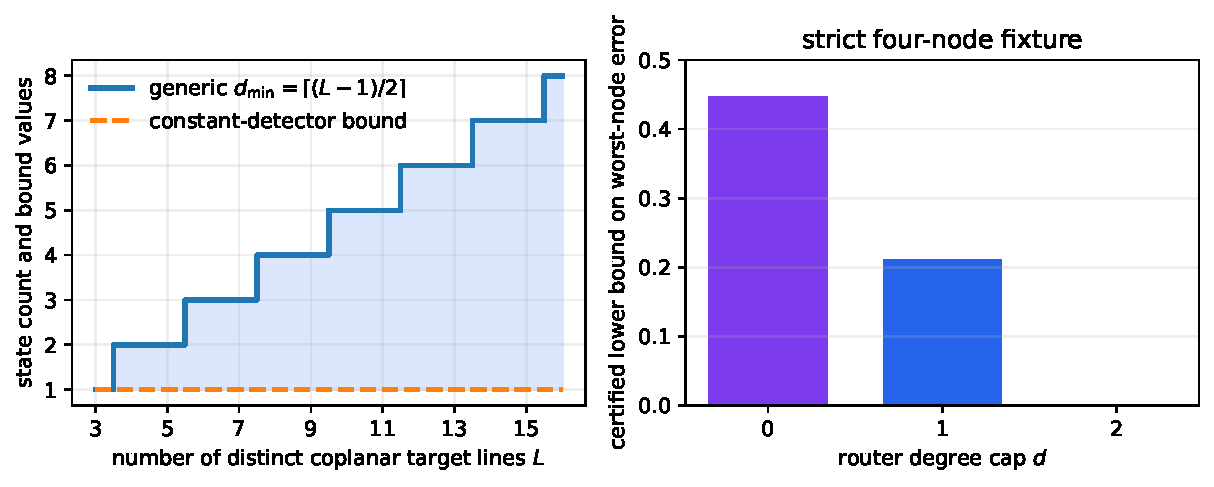
\includegraphics[width=0.75\linewidth]{figures/unbounded_detector_gap.pdf}
\caption{Generic exact memory on the coplanar distinct-target stratum versus
the constant-detector lower bound.  The separation corresponds to an unbounded
multiplicative ratio.}
\label{fig:gap}
\end{figure}

\section{The complete four-line phase diagram}

For four ordered distinct nodes, write
\[
 [z_1,z_2;z_3,z_4]
 =\frac{(z_1-z_3)(z_2-z_4)}{(z_1-z_4)(z_2-z_3)}
\]
with the usual projective conventions at infinity.  The order matters because
each frequency is paired with a specified target.
The projective classification below is classical/elementary; our claim is its
exact consequence for square passive rational-inner routers.

\begin{theorem}[Four-line classification]\label{thm:four}
For four target lines in one two-plane, the exact passive memory is
\begin{equation}\label{eq:four}
d_{\min}=\begin{cases}
0,&\text{all four targets coincide},\\
1,&\text{all four are distinct and their ordered cross-ratio equals that of the nodes},\\
3,&\text{the target multiplicities are }3+1,\\
2,&\text{in every remaining case.}
\end{cases}
\end{equation}
\end{theorem}

\begin{proof}
A nonconstant degree-one map is a projective bijection, so it sends the four
nodes to four distinct targets and preserves their ordered cross-ratio.  These
conditions are also sufficient by the uniqueness of a projective map through
three ordered points.

If three nodes share a target and the fourth does not, a nonconstant map of
degree at most two cannot work because every fiber has at most two distinct
points.  Polynomial interpolation gives the universal upper bound three.

It remains to show degree at most two in all other nonconstant cases.  For four
distinct targets with mismatched cross-ratio, normalize domain and target triples
to $(0,\infty,1)$, leaving $s\mapsto t$ with $s\ne t$.  Then
\[
 R(z)=z(az+b),\qquad
 a=\frac{t-s}{s(s-1)},\quad b=1-a
\]
has degree two and realizes the data.  For multiplicities $2+2$, after choosing
a finite chart use
\[
 R(z)=c\frac{(z-z_1)(z-z_2)}{(z-z_3)(z-z_4)}.
\]
For $2+1+1$, normalize the repeated nodes to $0,\infty$, the other nodes to
$1,s$, and the targets to $\infty,\infty,0,1$.  Choose
$a\notin\{0,1,s\}$ and set
\[
 q(z)=z,\qquad p(z)=A(z-1)(z-a),\qquad
 A=\frac{s}{(s-1)(s-a)}.
\]
This is a coprime degree-two witness.  None of these cases is constant or
degree one, completing the lower bounds and the classification via
\cref{thm:planar}.
\end{proof}

\begin{example}[Strict detector failure]\label{ex:strict}
Take
\[
 (\zeta_1,\zeta_2,\zeta_3,\zeta_4)=(1,i,-1,-i),\qquad
 (Y_1,Y_2,Y_3,Y_4)=(0,1,\infty,2).
\]
The ordered cross-ratios are $2$ and $1/2$, respectively.  Hence
$d_{\min}=2$, while both constant lower bounds equal one.  An exact witness is
\[
 p(z)=-\frac{(z-1)(3z-i)}2,\qquad q(z)=z+1,
 \qquad \Res(p,q)=-3-i\ne0.
\]
It takes the four requested projective values exactly.
\end{example}

\section{Delay price and reproducibility}

For a differentiable lossless boundary response, define the Wigner--Smith
matrix
\[
                  Q(\theta)=-iS(e^{i\theta})^*
                             \frac{\dd}{\dd\theta}S(e^{i\theta}).
\]
Jacobi's formula gives
$\operatorname{tr}(S^{-1}\partial_\theta S)=\partial_\theta\log\det S$.
Together with Potapov's factorization and winding count, this gives
\[
             \int_0^{2\pi}\operatorname{tr}Q(\theta)\dd\theta
             =2\pi\,\mcdeg S
\]
for finite rational-inner $S$ \cite{Wigner1955,Smith1960}.  Combining it with
\cref{thm:planar} yields an exact action law.

\begin{corollary}[Optimal integrated delay]\label{cor:delay}
For every planar line-routing table,
\[
 \inf_S\int_0^{2\pi}\operatorname{tr}Q(\theta)\dd\theta=2\pi\delta.
\]
The explicit completion \eqref{eq:completion} attains the infimum.
\end{corollary}

The computational artifact uses exact arithmetic over $\mathbb Q(i)$.  It
checks the strict witness in Example~\ref{ex:strict}; exact representatives of the
constant, cross-ratio-compatible, $2+2$, $2+1+1$, and $3+1$ strata;
full-column-rank exclusions below the
generic threshold; coprime threshold witnesses for every $3\le L\le16$; and
every nontrivial binary occupancy split through $L=16$ (119 exact cases).
The frozen validator recomputes the content hash and checks declared coverage,
phase degrees, ranks, and bounds.  In CI the producer is replayed from scratch
and its byte-identical JSON is compared with the frozen record; this replay is
the algebraic check of cross-ratios, witness values, gcds, and resultants.
These calculations
audit examples and certificates; they are not substitutes for the proofs.

\begin{limitation}[Exact scope]
The theorem assumes distinct frequency nodes, one input line, target lines in
one common two-plane, free endpoint phases, and square finite rational-inner
competitors.  Repeated nodes require confluent interpolation.  Fixed frames,
higher-rank subspaces, lossy or active architectures, and a complete equality
theory for nonplanar singular arrangements are not claimed.
\end{limitation}

\begin{limitation}[Priority scope]
Scalar minimal rational interpolation, the generic half-degree threshold,
cross-ratio and fiber classifications, subspace Nevanlinna interpolation,
Fej\'er--Riesz/paraunitary completion, and matrix all-pass construction predate
this work.  We claim the passive-memory equality \eqref{eq:main}, obtained by
combining a standard exact-degree lossless lift with the escape-from-the-plane
lower bound, and its physical/detector consequences; we do not claim a new
general rational interpolation algorithm or priority for the scalar strata.
\end{limitation}

\paragraph{Immutable reproducibility record.}
The tagged release containing the paper, exact producer, frozen validator,
frozen JSON certificate, and figure is:
\begin{center}\small
\href{https://github.com/lluiseriksson/finite-sample-spectral-certificates/releases/tag/v3.0-planar-projective-memory}{GitHub release: \texttt{v3.0-planar-projective-memory}}
\end{center}

\section{Conclusion}

Coplanarity does not make passive routing cheap.  It changes the governing
invariant.  Once every target lies in a two-plane, the exact state count is the
degree of an ordered projective rational interpolant.  Fej\'er--Riesz lifting
turns that algebraic object into a lossless network without spending an extra
state, while a common-denominator argument proves that no smaller network can
escape the plane.  The result exposes a generic half-linear memory law in a
regime where the optimized constant-detector hierarchy reports one, classifies
the first nontrivial
cross-ratio strata completely, and identifies the same integer as optimal
integrated delay divided by $2\pi$.  It also marks the next frontier precisely:
higher-dimensional singular target varieties motivate detectors that move with
frequency, rather than merely more constant minors.

\bibliographystyle{unsrt}
\bibliography{references}
\end{document}
